\documentclass[conference]{IEEEtran}
\usepackage[T1]{fontenc}
\usepackage[utf8]{inputenc}
\usepackage[spanish,es-noshorthands,es-nodecimaldot]{babel}
\usepackage{graphicx,array,amsmath,xurl}
\usepackage[hidelinks]{hyperref}
\usepackage{xcolor,fancyhdr}
\definecolor{usbnaranja}{HTML}{ED7D31}
\fancypagestyle{usb}{\fancyhf{}\fancyhead[L]{\footnotesize PLATAFORMA PWA CON IA PARA LA PREVENCIÓN CARDIOVASCULAR}%
  \fancyhead[R]{\footnotesize\thepage}%
  \renewcommand{\headrule}{{\color{usbnaranja}\hrule height 0.8pt}}}
\addto\captionsspanish{\renewcommand{\tablename}{TABLA}}
\begin{document}
\title{Plataforma PWA con IA para la Prevención Cardiovascular: Predicción de Riesgo, Alimentación, Ejercicio y Seguimiento Personalizado}
\author{\IEEEauthorblockN{Agustín Peralta Guarín\\Natalia Moncaleano Montero}\IEEEauthorblockA{\textit{Facultad de Ingeniería, Ingeniería de Sistemas}\\\textit{Universidad de San Buenaventura}\\Bogotá, Colombia}}
\maketitle
\thispagestyle{usb}
\pagestyle{usb}
\begin{abstract}
Las enfermedades del sistema circulatorio constituyen la primera causa de mortalidad general en Colombia, con tasas ajustadas superiores a 130 muertes por cada 100.000 habitantes. Más de tres cuartas partes de esa carga se asocia a factores de riesgo modificables, de modo que existe una ventana de intervención preventiva que hoy no se aprovecha, principalmente porque el tamizaje cardiovascular depende de que la persona asista a consulta. Este proyecto desarrolla Pulso, una Aplicación Web Progresiva (PWA) con inteligencia artificial dirigida a personas adultas de 40 a 69 años residentes en Colombia, sin diagnóstico previo de enfermedad cardiovascular. El sistema estima el riesgo cardiovascular, genera recomendaciones alimenticias con ingredientes, cantidades y preparaciones ajustadas a la región, planes de vida saludable y rutinas de ejercicio, y hace seguimiento con reportes periódicos. La estimación del riesgo se realiza con una regresión logística entrenada sobre 5.043 adultos de la encuesta NHANES 2021-2023, seleccionada frente a gradient boosting y k vecinos más cercanos mediante validación cruzada estratificada 5 $\times$ 10. Con las variables de estilo de vida, la edad y el sexo alcanza un área bajo la curva ROC de 0{,}805 con pendiente de calibración de 0{,}99, y la contribución de cada variable a cada predicción se calcula de forma exacta, dado que en un modelo lineal el valor SHAP tiene forma cerrada. La inferencia se ejecuta en el servidor. Sin conexión, la aplicación conserva la última evaluación con su explicación, el plan alimentario, las rutinas y el histórico, mientras que una evaluación nueva se calcula al recuperar la conectividad. La validación prevista comprende métricas de discriminación y calibración, pruebas de usabilidad con la escala SUS en distintos dispositivos y condiciones de conectividad, y la revisión de un profesional de salud.
\end{abstract}
\renewcommand{\IEEEkeywordsname}{Palabras clave}
\begin{IEEEkeywords}
enfermedades cardiovasculares, aprendizaje automático, regresión logística, aplicación web progresiva, prevención primaria, salud digital
\end{IEEEkeywords}
\noindent\textbf{\textit{Abstract}---Circulatory system diseases are the leading cause of overall mortality in Colombia, with age-adjusted rates above 130 deaths per 100{,}000 inhabitants. More than three quarters of that burden is associated with modifiable risk factors, which leaves a window for preventive intervention that is currently missed, mainly because cardiovascular screening depends on the person attending a medical appointment. This project develops Pulso, an artificial intelligence Progressive Web Application (PWA) aimed at adults aged 40 to 69 living in Colombia with no prior diagnosis of cardiovascular disease. The system estimates cardiovascular risk, generates dietary recommendations with ingredients, quantities and preparations adjusted to each region, healthy lifestyle plans and exercise routines, and supports follow-up with periodic reports. Risk is estimated with a logistic regression trained on 5{,}043 adults from the NHANES 2021-2023 survey, selected against gradient boosting and k-nearest neighbours through 5 $\times$ 10 stratified cross-validation. With lifestyle variables, age and sex it reaches an area under the ROC curve of 0.805 with a calibration slope of 0.99, and the contribution of each variable to each prediction is computed exactly, since SHAP values have a closed form for linear models. Inference runs on the server. Offline, the application keeps the latest evaluation with its explanation, the meal plan, the routines and the history, while a new evaluation is computed once connectivity is restored. The planned validation covers discrimination and calibration metrics, usability tests with the SUS scale across devices and connectivity conditions, and a review by a health professional.}

\noindent\textbf{\textit{Keywords}---cardiovascular diseases, machine learning, logistic regression, progressive web application, primary prevention, digital health}

\section{Introducción}
Las enfermedades cardiovasculares (ECV) constituyen la primera causa de mortalidad en Colombia. Las enfermedades del sistema circulatorio encabezan de forma sostenida las estadísticas nacionales de mortalidad general, con tasas ajustadas superiores a 130 muertes por cada 100.000 habitantes según los reportes del Ministerio de Salud y Protección Social [1]. Este comportamiento reproduce, a escala nacional, un fenómeno global: la Organización Mundial de la Salud estima cerca de 19{,}8 millones de muertes anuales por esta causa, alrededor del 32 \% de las defunciones registradas en el mundo [2], mientras que el World Heart Report 2023 de la World Heart Federation calcula 20{,}5 millones de muertes para el año 2021 [3].

Ahora bien, la magnitud del problema no es su rasgo más determinante. Más de tres cuartas partes de la carga atribuible a estas enfermedades se asocia a factores de riesgo modificables, tales como el sedentarismo, la alimentación inadecuada, el tabaquismo, la obesidad y el estrés. Existe, por consiguiente, una ventana de intervención amplia que en el contexto colombiano no se aprovecha.

El obstáculo se ubica en el momento de la detección. El tamizaje cardiovascular disponible en el país opera de forma reactiva, pues depende de que la persona asista a consulta y de que un profesional aplique una escala de riesgo durante la atención. En consecuencia, una proporción significativa de la población adulta desconoce su nivel de riesgo hasta que ocurre un evento agudo como el infarto de miocardio o el accidente cerebrovascular, momento en el cual la intervención deja de ser preventiva. La situación se agrava por la desigualdad territorial: en municipios rurales y dispersos la oferta de servicios preventivos es menor y la conectividad resulta intermitente.

Desde la ingeniería de sistemas es posible abordar esta situación mediante el desarrollo de aplicaciones web progresivas inteligentes que analicen datos clínicos y de estilo de vida del usuario, calculen su nivel de riesgo cardiovascular y generen planes de acción personalizados. La elección de la arquitectura de Aplicación Web Progresiva (PWA) responde a la necesidad de ofrecer una experiencia equivalente a la de una aplicación nativa en cualquier dispositivo con navegador web, sin depender de tiendas de aplicaciones, con capacidad de funcionamiento sin conexión y envío de notificaciones push para alertas de salud críticas.

Las tecnologías emergentes como la inteligencia artificial y el aprendizaje automático han demostrado un alto potencial para mejorar la precisión en la estratificación del riesgo cardiovascular y la personalización de intervenciones preventivas [4], [5]. Pulso integra estas tecnologías en una PWA dirigida a personas adultas entre 40 y 69 años residentes en Colombia, sin diagnóstico previo de enfermedad cardiovascular y con acceso a un dispositivo con navegador web, que no solo predice el riesgo, sino que ofrece recomendaciones alimenticias con ingredientes específicos, planes de vida saludable y rutinas de ejercicio adaptadas.

Este documento analiza las limitaciones existentes y propone un enfoque viable para el diseño de una PWA inteligente orientada a la prevención cardiovascular integral en el contexto colombiano, mediante datos y recomendaciones contextualizadas por región, cultura alimentaria y disponibilidad de ingredientes locales.

\section{Planteamiento del problema}
Las enfermedades cardiovasculares constituyen la primera causa de mortalidad general en Colombia y su comportamiento no responde a un déficit de conocimiento clínico, sino a una falla en el momento de la detección. Más del 75\% de la carga atribuible a estas enfermedades se asocia a factores de riesgo modificables, lo que implica que existe una ventana de intervención amplia que actualmente no se aprovecha.

El tamizaje cardiovascular disponible opera de forma reactiva: depende de que la persona asista a consulta y de que un profesional aplique una escala de riesgo durante la atención. Quien no consulta, no se tamiza. Como consecuencia, una proporción significativa de la población adulta desconoce su nivel de riesgo hasta que ocurre un evento clínico agudo, momento en el cual la intervención deja de ser preventiva.

La situación adquiere un matiz territorial. En los municipios rurales y dispersos del país la oferta de servicios preventivos es menor, la conectividad es intermitente y los dispositivos disponibles son de gama baja, de modo que la brecha de detección no se distribuye de manera uniforme sobre el territorio nacional.

A esta condición se suma una limitación tecnológica. Las herramientas digitales existentes fueron diseñadas para entornos hospitalarios, requieren conexión permanente, entregan un porcentaje de riesgo sin plan de acción asociado y distribuyen en aplicaciones independientes lo que el usuario necesita de forma integrada. Por consiguiente, quedan excluidas precisamente las poblaciones con mayor barrera de acceso y mayor carga de enfermedad.

El presente trabajo delimita su población objetivo en personas adultas entre 40 y 69 años residentes en Colombia, sin diagnóstico previo de enfermedad cardiovascular y con acceso a un dispositivo con navegador web. El rango etario no es arbitrario: corresponde al intervalo en el que están validadas las escalas de riesgo cardiovascular a diez años de referencia, como SCORE2, desarrollada específicamente para personas aparentemente sanas de 40 a 69 años [6]. Por debajo de los 40 años la estimación a diez años tiende a subestimar el riesgo de por vida, y por encima de los 69 el manejo corresponde al ámbito clínico y no al autotamizaje.

La situación problema se manifiesta en cuatro dimensiones observables. En primer lugar, el diagnóstico tardío, dado que el tamizaje se concentra en el nivel asistencial y la primera señal de alerta termina siendo el evento agudo. En segundo lugar, la fragmentación de la orientación preventiva, puesto que las calculadoras de riesgo entregan un porcentaje sin plan de acción asociado, las aplicaciones de nutrición no consideran el perfil de riesgo cardiovascular y las de ejercicio no incorporan alertas de seguridad según el nivel de riesgo. En tercer lugar, la brecha de accesibilidad tecnológica, en tanto las plataformas existentes requieren descarga desde tiendas de aplicaciones, consumen almacenamiento del dispositivo y no operan sin conexión. En cuarto lugar, la descontextualización de las recomendaciones, ya que las guías nutricionales de referencia se formulan sobre patrones alimentarios de países de altos ingresos y una recomendación que no considera la disponibilidad local de ingredientes, el costo relativo ni la cultura alimentaria colombiana tiene baja probabilidad de adherencia.

El interrogante que orienta esta investigación es:

\textit{¿De qué manera una Aplicación Web Progresiva impulsada por inteligencia artificial puede contribuir a la predicción, prevención y reducción del riesgo cardiovascular en personas adultas entre 40 y 69 años en Colombia, mediante recomendaciones personalizadas y contextualizadas de alimentación, ejercicio y hábitos de vida saludable?}

\subsection{Antecedentes}
Los antecedentes que sustentan este proyecto se organizan en cuatro campos que han evolucionado de manera independiente: la predicción del riesgo cardiovascular mediante aprendizaje automático, la nutrición computacional, la prescripción asistida de actividad física y la arquitectura de aplicaciones web progresivas aplicada a la salud.

En cuanto a la predicción del riesgo, Weng et al. [5] evaluaron cuatro algoritmos sobre registros clínicos rutinarios de 378.256 pacientes de atención primaria del Reino Unido y encontraron que todos superaron el desempeño del algoritmo de referencia del American College of Cardiology, con un incremento del 7{,}6\% en el número de pacientes correctamente identificados por el modelo de redes neuronales. El resultado es relevante porque demuestra que la ganancia predictiva no proviene de datos especializados de difícil obtención, sino de un mejor aprovechamiento de variables clínicas ya disponibles. Debe advertirse, no obstante, que el estudio se realizó sobre población británica, por lo cual la transferencia de sus resultados al contexto colombiano requiere validación posterior. En la misma línea, Krittanawong et al. [4] realizaron un metaanálisis sobre la predicción de eventos cardiovasculares con técnicas de aprendizaje automático y reportaron desempeños comparables o superiores a los de las escalas clínicas tradicionales, señalando al mismo tiempo la heterogeneidad metodológica y la escasa validación externa como limitaciones persistentes del campo. Esta observación sustenta la decisión de incorporar mecanismos de explicabilidad al modelo propuesto.

En nutrición computacional, Zeevi et al. [7] demostraron que la respuesta glucémica a un mismo alimento varía de manera significativa entre individuos y que un modelo predictivo alimentado con datos personales permite diseñar intervenciones alimentarias con resultados clínicamente medibles. Este antecedente evidencia que la recomendación nutricional genérica tiene un techo de efectividad y que la personalización no constituye un valor agregado opcional sino una condición del resultado.

Respecto de la prescripción de actividad física asistida por sistemas de recomendación, diversos trabajos han explorado la generación automática de planes adaptados al perfil del usuario; Liao et al. [8] mostraron que un algoritmo que personaliza las sugerencias de actividad a partir de los datos de cada persona puede optimizar la actividad física diaria frente a sugerencias no personalizadas. Para el caso cardiovascular, la literatura enfatiza la necesidad de incorporar límites de seguridad y progresividad controlada, dado que una prescripción inadecuada en población de alto riesgo puede resultar contraproducente.

En materia de aplicaciones web progresivas aplicadas a la salud, Biduski et al. [9] analizaron la experiencia de uso a largo plazo en una aplicación móvil de salud y documentaron que las experiencias más satisfactorias se concentran en las primeras semanas, con una caída posterior sostenida. Este hallazgo refuerza la importancia del seguimiento activo y de las notificaciones como mecanismo de retención. En cuanto a la arquitectura, la literatura reporta ventajas de las PWA frente a las aplicaciones nativas en contextos de salud pública: la no dependencia de tiendas de aplicaciones, el menor consumo de almacenamiento, las actualizaciones transparentes y el mantenimiento de la funcionalidad ante conectividad intermitente mediante Service Workers.

En el contexto nacional, los reportes del Ministerio de Salud y Protección Social [1] ubican las enfermedades del sistema circulatorio como primera causa de mortalidad general, y la literatura ha identificado barreras estructurales que incluyen la baja cobertura de tamizaje en población general, las desigualdades entre las ciudades capitales y los municipios rurales en el acceso a servicios preventivos y la limitada adopción tecnológica en atención primaria. No se identificaron herramientas digitales de autotamizaje cardiovascular dirigidas a la población adulta colombiana que operen sin conexión y entreguen recomendaciones alimentarias ajustadas a la disponibilidad regional de ingredientes.

En conjunto, los antecedentes revisados muestran componentes maduros de forma aislada: modelos predictivos validados sobre grandes cohortes, nutrición personalizada con evidencia clínica, sistemas de recomendación de actividad física y arquitectura PWA probada en contextos de salud pública. Sin embargo, no se identificó una plataforma que articule estos componentes en un solo flujo de uso, de acceso libre, funcional sin conexión y con recomendaciones contextualizadas por región y cultura alimentaria. Ese es el vacío que aborda el presente proyecto.

\section{Justificación}
\subsection{Relevancia social}
Las enfermedades cardiovasculares no representan únicamente un problema de salud pública, sino también un indicador de desigualdad social. En Colombia, buena parte de la población adulta carece de acceso oportuno a servicios de salud preventivos, lo que incrementa las tasas de mortalidad por eventos evitables. El desarrollo de Pulso como aplicación de acceso libre democratiza el acceso a herramientas de evaluación del riesgo cardiovascular, orientación nutricional con ingredientes específicos y recomendaciones de vida saludable, y contribuye a reducir la brecha de detección entre las ciudades capitales y el resto del territorio.

La arquitectura de aplicación web progresiva resulta especialmente pertinente para el contexto colombiano, donde la conectividad a internet es desigual entre regiones y predomina el acceso mediante dispositivos móviles de gama media y baja. La capacidad de funcionamiento sin conexión permite que usuarios de municipios rurales o con acceso limitado consulten su último nivel de riesgo calculado, sus recomendaciones alimenticias y sus rutinas de ejercicio sin necesidad de una conexión permanente.

\subsection{Relevancia teórica}
La investigación se apoya en estudios que demuestran la efectividad de la inteligencia artificial en la estratificación del riesgo cardiovascular y en la personalización de intervenciones preventivas [4], [5]. Desde la ingeniería de sistemas, este trabajo fortalece la base teórica sobre el uso de tecnologías web progresivas inteligentes integradas con sistemas de información en salud, y aporta al campo de la salud digital, la nutrición computacional y la medicina preventiva de precisión.

\subsection{Relevancia práctica}
La aplicación propuesta permitirá a las personas adultas entre 40 y 69 años residentes en Colombia ingresar sus datos clínicos y de estilo de vida para obtener una estimación personalizada de su riesgo cardiovascular, calculada con una regresión logística entrenada sobre una encuesta poblacional y acompañada de la contribución de cada variable; recomendaciones alimenticias detalladas con ingredientes específicos, cantidades, métodos de preparación y alternativas según la región del país y la cultura alimentaria del usuario; planes de vida saludable que integren manejo del estrés, calidad del sueño, hidratación y hábitos de descanso; rutinas de ejercicio adaptadas a su condición física, nivel de riesgo y objetivos personales; alertas preventivas automáticas mediante notificaciones push; y reportes periódicos configurables, accesibles sin conexión, que permitan visualizar la evolución de sus indicadores.

\subsection{Relevancia disciplinar}
Desde la formación en ingeniería de sistemas, el proyecto articula competencias de arquitectura de software, ciencia de datos, desarrollo web y diseño de experiencia de usuario en torno a un problema de salud pública con evidencia epidemiológica verificable. La restricción de operar sin conexión y sobre dispositivos de gama baja obliga a decisiones de diseño no triviales sobre el almacenamiento local, la sincronización y la ubicación de la inferencia del modelo, lo que constituye en sí mismo un aporte metodológico replicable en otros dominios de salud digital.

\section{Alcance y limitaciones}
El presente proyecto tiene como alcance el desarrollo de Pulso, una Aplicación Web Progresiva basada en inteligencia artificial y aprendizaje automático, orientada a la estimación del riesgo cardiovascular, la generación de recomendaciones alimenticias con ingredientes específicos, planes de vida saludable, rutinas de ejercicio personalizadas y el seguimiento continuo del estado de salud cardiovascular del usuario. El sistema será instalable en dispositivos móviles, tabletas y equipos de escritorio, mantendrá disponibles sin conexión las funciones de consulta mediante Service Workers y enviará notificaciones push para alertas preventivas.

\subsection{Población objetivo}
La población objetivo del proyecto son las personas adultas entre 40 y 69 años residentes en Colombia, sin diagnóstico previo de enfermedad cardiovascular y con acceso a un dispositivo con navegador web. Cada criterio responde a una razón concreta.

\begin{itemize}
\item El rango de 40 a 69 años corresponde al intervalo en el que están validadas las escalas de riesgo cardiovascular a diez años que sirven de referencia al modelo. Por debajo de los 40 años la estimación a diez años tiende a subestimar el riesgo acumulado a lo largo de la vida, y por encima de los 69 el manejo corresponde al ámbito clínico especializado.
\item La ausencia de diagnóstico previo delimita el proyecto a la prevención primaria. Las personas que ya presentaron un evento cardiovascular requieren seguimiento clínico y no autotamizaje, por lo cual quedan fuera de la población objetivo.
\item La residencia en Colombia permite contextualizar las recomendaciones alimenticias según la disponibilidad regional de ingredientes y la cultura alimentaria del país, y alinear el sistema con el marco normativo nacional de protección de datos personales.
\item El acceso a un dispositivo con navegador web es la condición material de uso del sistema. Las personas que no cuentan con ese acceso no pueden ser atendidas por esta solución, y ello constituye una limitación estructural reconocida del proyecto.
\end{itemize}
\subsection{Módulos comprendidos en el alcance}
\begin{itemize}
\item Ingreso de datos clínicos y de estilo de vida con almacenamiento local mediante IndexedDB.
\item Estimación del riesgo cardiovascular mediante una regresión logística entrenada sobre la encuesta NHANES 2021-2023 [10], seleccionada frente a gradient boosting y k vecinos más cercanos, con explicación de cada predicción mediante valores SHAP calculados de forma exacta. El conjunto UCI Heart Disease se usa para verificar la implementación, y el Framingham Heart Study y el WHO Global Health Observatory como fundamento bibliográfico de los factores de riesgo, no como corpus de entrenamiento.
\item Recomendaciones alimenticias personalizadas con ingredientes específicos, cantidades, métodos de preparación, alternativas según la región del país y planes semanales con lista de mercado consolidada.
\item Recomendaciones de vida saludable que abarcan manejo del estrés, calidad del sueño, hidratación y hábitos cotidianos.
\item Rutinas de ejercicio adaptadas al nivel de riesgo, con progresividad automática y alertas de seguridad.
\item Sistema de seguimiento con tablero interactivo, alertas preventivas y reportes periódicos exportables en PDF.
\end{itemize}
\subsection{Vigencia y naturaleza temporal de los datos}
El proyecto trabaja con dos tipos de datos que tienen vigencias distintas y no deben confundirse. Los datos epidemiológicos que sustentan el planteamiento del problema corresponden al periodo 2021-2023. La cifra de 20{,}5 millones de muertes por enfermedad cardiovascular refleja el año 2021 y fue publicada en el World Heart Report 2023 de la World Heart Federation [3]. Se trata, por tanto, de la evidencia disponible más reciente sobre la magnitud del problema.

El conjunto de entrenamiento del modelo es la encuesta NHANES del ciclo agosto de 2021 a agosto de 2023, publicada en 2024 [10], que coincide en periodo con la evidencia epidemiológica. El conjunto UCI Heart Disease [11], recolectado en 1988, se emplea únicamente para verificar que la implementación de los algoritmos reproduce resultados conocidos. El Framingham Heart Study no se usa como corpus, porque el acceso a sus datos individuales exige aprobación de un comité de ética y un acuerdo de uso, y el WHO Global Health Observatory publica solo agregados por país; ambos sustentan los factores de riesgo desde la literatura [12]. De lo anterior se derivan dos precisiones: la estimación debe entenderse como un nivel de riesgo derivado de patrones poblacionales y no como una medición del estado clínico presente del usuario, y el modelo se entrena sobre población estadounidense, por lo cual la revalidación con datos poblacionales colombianos queda planteada como línea de trabajo posterior.

\subsection{El sistema no opera en tiempo real}
Pulso es un sistema de evaluación periódica y no de monitoreo continuo. Esta decisión es deliberada y responde a cuatro razones. En primer lugar, la fuente de información es el autorreporte: el usuario ingresa manualmente sus datos clínicos y de estilo de vida, de modo que la frecuencia de actualización depende de él y no de un flujo automático. En segundo lugar, el sistema no se integra con dispositivos vestibles, sensores biométricos ni con historias clínicas electrónicas, pues dicha interoperabilidad exigiría estándares de intercambio clínico y acuerdos institucionales que exceden el alcance de un prototipo académico. En tercer lugar, la arquitectura sin conexión implica que los datos residen localmente en el navegador mediante IndexedDB y se sincronizan cuando hay conectividad disponible. En cuarto lugar, un sistema de monitoreo continuo con alertas clínicas inmediatas se aproximaría a la categoría de dispositivo médico y quedaría sujeto a un régimen regulatorio que este proyecto no aborda.

Por lo anterior, el nivel de riesgo que muestra la aplicación corresponde siempre al último registro ingresado por el usuario, y las alertas push cumplen una función de recordatorio y de estímulo a la reevaluación periódica, no de detección de eventos agudos. La aplicación no debe utilizarse como mecanismo de vigilancia ante una urgencia cardiovascular.

\subsection{Limitaciones}
El proyecto presenta limitaciones derivadas del acceso restringido a bases de datos clínicas reales de pacientes por motivos éticos y de confidencialidad, razón por la cual se emplearán conjuntos de datos públicos y anonimizados para el entrenamiento de los modelos. El desarrollo se limitará a un prototipo funcional en fase experimental, sin implementación directa en instituciones médicas, y su validación se centrará en métricas computacionales de desempeño y en pruebas de usabilidad con usuarios representativos.

Una limitación de especial importancia se deriva de la delimitación nacional del proyecto. El conjunto de entrenamiento proviene de población estadounidense y no colombiana, y aplicar a un contexto nacional un modelo aprendido sobre una población con perfiles demográficos, dietarios y de acceso a servicios de salud distintos puede introducir un sesgo sistemático en la estimación del riesgo. A ello se suman tres límites propios de la encuesta que se declaran de forma explícita: su diseño es transversal, de modo que permite estimar la asociación con el antecedente de un evento cardiovascular pero no la incidencia futura; el desenlace es autorreportado; y el estrés se aproxima con el cuestionario PHQ-9 [13], que mide síntomas depresivos y no estrés percibido. El proyecto mitiga parcialmente estas limitaciones mediante la explicación por variable y la declaración del carácter orientativo del resultado, pero no las elimina; la validación con datos poblacionales colombianos queda planteada como condición para cualquier uso más allá del prototipo académico.

Adicionalmente, las recomendaciones generadas por la aplicación son de carácter orientativo y no sustituyen el criterio médico profesional; la disponibilidad de ingredientes puede variar según la región del país; las funcionalidades sin conexión dependen del soporte que cada navegador ofrezca para Service Workers e IndexedDB; una evaluación nueva requiere conectividad, porque la inferencia se ejecuta en el servidor; y la precisión del modelo estará condicionada por la calidad y veracidad de los datos ingresados, dado que el sistema no cuenta con mecanismos de verificación clínica directa.

\subsection{Operación sin conexión y ubicación de la inferencia}
La estimación del riesgo y el cálculo de su explicación se ejecutan en el servidor y no en el navegador. La decisión responde a tres razones: garantiza que cada evaluación registre la versión exacta del modelo que la produjo, mantiene una sola copia del modelo sin distribuir lógica en el cliente y permite reentrenar o sustituir el modelo sin modificar la aplicación instalada. En consecuencia, la aplicación no calcula evaluaciones nuevas sin conexión; lo que sí garantiza sin red es el acceso a la última evaluación con su explicación y a las recomendaciones ya generadas, como se detalla en la tabla siguiente.

\begin{table*}[!t]
\centering
\caption{Comportamiento de las funciones de pulso según la conectividad}
\footnotesize
\renewcommand{\arraystretch}{1.15}
\begin{tabular}{>{\raggedright\arraybackslash}p{0.383\linewidth}>{\raggedright\arraybackslash}p{0.131\linewidth}>{\raggedright\arraybackslash}p{0.376\linewidth}}
\hline
\textbf{Función} & \textbf{Con conexión} & \textbf{Sin conexión} \\ \hline
Consultar la última evaluación y la contribución de cada variable & Disponible & Disponible, desde la copia local en IndexedDB \\ \hline
Registrar datos clínicos y de estilo de vida & Se envían y se evalúan de inmediato & Se guardan en la cola local y se evalúan al reconectar \\ \hline
Calcular una evaluación nueva del riesgo & Disponible, en el servidor & No disponible; la aplicación lo indica al usuario \\ \hline
Consultar plan alimentario, lista de mercado, rutinas y hábitos & Disponible & Disponible, desde la caché del Service Worker \\ \hline
Generar un plan alimentario o una rutina nuevos & Disponible & No disponible \\ \hline
Consultar el histórico y exportar el reporte PDF & Disponible & Disponible con los datos sincronizados hasta la última conexión \\ \hline
Recibir notificaciones push & Disponible & Se entregan cuando el dispositivo recupera la conexión \\ \hline
\end{tabular}
\par\smallskip\parbox{\linewidth}{\scriptsize\textit{Nota:} elaboración propia.}
\end{table*}
La explicación no requiere ejecutar el modelo en el dispositivo porque se calcula junto con la predicción y se almacena con ella. Como el modelo seleccionado es lineal en la escala logit, el valor SHAP de cada variable se obtiene en forma cerrada, sin el muestreo que exigen los métodos genéricos de explicación [14]. Esto resuelve la aparente contradicción entre operación sin conexión y explicabilidad: la explicación de un resultado existe desde el momento en que el resultado existe. Dado que el modelo consta de siete coeficientes y un intercepto, su ejecución en el navegador es técnicamente factible y queda planteada como mejora posterior para permitir evaluaciones completamente sin conexión.

\section{Objetivos}
\subsection{Objetivo general}
Desarrollar Pulso, una Aplicación Web Progresiva basada en inteligencia artificial para la predicción del riesgo cardiovascular, la generación de recomendaciones alimenticias con ingredientes específicos, planes de vida saludable, rutinas de ejercicio personalizadas y seguimiento continuo, dirigida a personas adultas entre 40 y 69 años residentes en Colombia sin diagnóstico previo de enfermedad cardiovascular.

\subsection{Objetivos específicos}
Para alcanzar el objetivo general se formulan los siguientes objetivos específicos, derivados de las causas raíz priorizadas en el planteamiento del problema:

\textit{1)} Diseñar la arquitectura de Pulso como Aplicación Web Progresiva y seleccionar el modelo de estimación del riesgo cardiovascular entre regresión logística, gradient boosting y k vecinos más cercanos, entrenados sobre la encuesta NHANES 2021-2023, justificando la elección por su discriminación, su calibración y su interpretabilidad, y definiendo qué funciones operan sin conexión mediante Service Workers e IndexedDB y dónde se ejecuta la inferencia.

\textit{2)} Desarrollar los módulos funcionales de Pulso, a saber, estimación del riesgo con el modelo seleccionado y explicación de cada predicción mediante valores SHAP calculados de forma exacta, recomendaciones alimenticias con ingredientes específicos y alternativas según la región del país, planes de vida saludable, rutinas de ejercicio con progresividad automática y sistema de seguimiento con tablero de evolución y reportes exportables en PDF.

\textit{3)} Validar el prototipo mediante métricas de desempeño del modelo (área bajo la curva ROC, calibración, sensibilidad y especificidad en el umbral operativo), pruebas de usabilidad con la escala SUS con usuarios representativos en distintos dispositivos y condiciones de conectividad, y la revisión de pertinencia clínica por parte de un profesional de salud.

\section{Metodología}
Este apartado distingue dos cosas que suelen confundirse. La metodología de investigación responde a cómo se estudia y se evalúa el problema; el marco de desarrollo responde a cómo se construye la solución técnica. Ambas conviven en el proyecto y emplean instrumentos distintos. A continuación se presentan las dos, seguidas del tratamiento que recibirán los datos personales, el procedimiento de preparación y limpieza de los conjuntos de datos y el plan de pruebas.

\subsection{Metodología de investigación}
El enfoque de investigación adoptado es mixto, en tanto combina la medición cuantitativa del desempeño con la interpretación cualitativa de la pertinencia y la experiencia de uso. La decisión no es una preferencia metodológica sino una consecuencia de la pregunta formulada: establecer de qué manera la aplicación contribuye a la predicción y prevención del riesgo exige tanto números como juicio experto, y ninguno de los dos componentes responde la pregunta por separado.

El componente cuantitativo permite establecer si el sistema funciona: el desempeño del modelo predictivo sobre el conjunto de prueba, los puntajes de usabilidad, las métricas de finalización de tareas y el cumplimiento de los criterios técnicos de aplicación web progresiva son magnitudes verificables y comparables. El componente cualitativo permite establecer si el sistema sirve: la pertinencia clínica de una recomendación alimenticia, la seguridad de una rutina de ejercicio para una persona con riesgo alto o la razón por la cual un usuario abandona un formulario no se obtienen de un promedio, sino de la revisión de un profesional de salud y de la observación directa durante las pruebas.

Según la clasificación por tipo de pregunta, la investigación es de carácter evaluativo o aplicado, dado que no busca caracterizar un fenómeno ni establecer una correlación, sino determinar en qué medida una solución propuesta produce el efecto esperado sobre un problema previamente delimitado.

Los instrumentos de recolección previstos son los siguientes:

\begin{itemize}
\item Benchmarking de las herramientas digitales de tamizaje cardiovascular existentes, contrastadas frente a los criterios de acceso libre, funcionamiento sin conexión, integración de recomendaciones y contextualización regional. Sustenta el vacío identificado en los antecedentes.
\item Métricas de desempeño de los modelos candidatos (área bajo la curva ROC, puntaje de Brier, calibración, sensibilidad y especificidad), obtenidas por validación cruzada estratificada, como instrumento cuantitativo principal de evaluación del primer y segundo objetivo específico.
\item Cuestionario estandarizado de usabilidad, la escala SUS [15], aplicado a usuarios representativos del rango de 40 a 69 años, complementado con el registro de tasa de finalización, tiempo por tarea y errores cometidos.
\item Listas de verificación técnica, empleadas para auditar el cumplimiento de los criterios de aplicación web progresiva y de los controles de seguridad definidos.
\item Entrevista semiestructurada a un profesional de salud, orientada a valorar la pertinencia y la seguridad de las recomendaciones alimenticias y de las rutinas de ejercicio.
\item Observación directa con notas de campo durante las sesiones de prueba de usabilidad, para registrar dificultades que el cuestionario no captura.
\end{itemize}
La muestra prevista para las pruebas de usabilidad es de entre diez y quince usuarios, cantidad suficiente para identificar la mayoría de los problemas de usabilidad relevantes en una evaluación de este tipo. No se trata de una muestra estadísticamente representativa de la población objetivo, y esa limitación se declara de forma explícita: el propósito es detectar defectos de interacción, no estimar parámetros poblacionales.

\subsection{Validación de los instrumentos}
Un instrumento no se aplica sin validarse previamente. La aplicación de un cuestionario mal formulado produce datos que parecen válidos y no lo son, y ese defecto no se detecta durante el análisis. El proyecto contempla tres mecanismos de validación, ajustados a la naturaleza de cada instrumento.

\subsubsection{Juicio de expertos}
El cuestionario de usabilidad y el guion de la entrevista al profesional de salud se someten a revisión por parte de dos o tres personas con experiencia en el área antes de su aplicación. La revisión evalúa tres criterios: pertinencia de cada ítem respecto del objetivo que pretende medir, claridad de la redacción para la población objetivo y suficiencia del conjunto de ítems para cubrir la dimensión evaluada. Las observaciones recibidas y los ajustes aplicados se documentan como evidencia del proceso.

\subsubsection{Prueba piloto}
Los instrumentos revisados se aplican a una muestra pequeña de entre tres y cinco personas, con el propósito de detectar preguntas ambiguas, problemas de comprensión del vocabulario técnico y fallas operativas en la sesión de prueba, tales como tareas mal enunciadas o tiempos de sesión mal estimados. Los participantes del piloto no se incluyen en la muestra final.

\subsubsection{Confiabilidad}
Para el cuestionario de usabilidad, que es un instrumento cuantitativo de escala, se calcula el coeficiente alfa de Cronbach como medida de consistencia interna. Un valor superior a 0{,}7 se considera aceptable. En caso de obtener un valor inferior, se revisan los ítems con menor correlación con el total antes de reportar cualquier resultado derivado del instrumento.

\subsubsection{Validación de los instrumentos técnicos}
Los instrumentos de carácter técnico, como las auditorías de rendimiento y cumplimiento de criterios de aplicación web progresiva, las listas de verificación de seguridad y las mediciones de desempeño del modelo, no admiten validación por juicio de expertos ni por consistencia interna. Su validación consiste en la repetibilidad: cada medición se ejecuta varias veces bajo condiciones controladas y equivalentes, y se verifica que los resultados sean consistentes entre ejecuciones. En el caso del modelo predictivo, la validación cruzada cumple esa función, dado que evita que el desempeño reportado dependa de una partición particular de los datos.

\subsection{Marco de desarrollo de la solución}
La construcción del sistema se realiza combinando Kanban y Programación Extrema (XP). De Kanban se adopta la gestión visual del flujo de trabajo, la limitación del trabajo en curso y las métricas de tiempo de ciclo, que permiten mantener un ritmo sostenido en un equipo reducido y evidenciar los cuellos de botella sin imponer la estructura de sprints. De XP se adoptan las prácticas de ingeniería que sostienen la calidad del código: iteraciones cortas con entregas funcionales, desarrollo guiado por pruebas, revisión cruzada del código, integración continua y refactorización permanente.

Los instrumentos de este marco son distintos de los de la investigación: un backlog de producto derivado de los módulos definidos en el alcance, historias de usuario con criterios de aceptación verificables, un tablero Kanban con límites de trabajo en curso y una definición de terminado, wireframes y mockups para el diseño de interfaz, diagramas UML de clases y de casos de uso, el modelo entidad-relación de la base de datos y un flujo de integración continua.

El criterio rector es la trazabilidad. Cada incremento debe poder rastrearse hasta un requisito, ese requisito hasta una de las causas priorizadas en el planteamiento del problema y esa causa hasta uno de los objetivos específicos, de modo que ninguna funcionalidad se incorpore sin justificación en el análisis del problema.

\subsection{Tratamiento de datos personales}
El proyecto adopta el principio de privacidad desde el diseño. La decisión de mantener los datos en el dispositivo del usuario mediante IndexedDB no obedece únicamente al funcionamiento sin conexión: constituye también la principal medida de protección de la privacidad, puesto que reduce el volumen de datos sensibles que salen del control directo del titular.

El tratamiento se rige por la Ley 1581 de 2012 y sus normas reglamentarias, cuyo cumplimiento vigila la Superintendencia de Industria y Comercio. Los datos clínicos y de estilo de vida constituyen datos sensibles, lo que implica que su tratamiento exige autorización explícita del titular y que ningún dato puede recolectarse por defecto.

De lo anterior se derivan las siguientes reglas de tratamiento:

\begin{itemize}
\item Minimización: se recolectan únicamente los datos estrictamente necesarios para estimar el riesgo y generar recomendaciones.
\item Consentimiento: la autorización para el tratamiento de datos sensibles se solicita de forma separada del registro y puede revocarse en cualquier momento.
\item Transparencia: la política de tratamiento de datos está disponible dentro de la aplicación, redactada en lenguaje comprensible para una persona sin formación jurídica.
\item Portabilidad y supresión: el usuario puede exportar la totalidad de sus datos en un formato legible por máquina, y la eliminación de la cuenta suprime los datos del dispositivo y del servidor con confirmación explícita.
\item No cesión: el sistema no comparte datos identificables con terceros ni incorpora servicios de analítica que transmitan información de salud.
\item Reentrenamiento: cualquier uso de datos para reentrenar el modelo se realiza sobre información anonimizada y previa autorización específica del titular.
\item Conservación: se define y se comunica un periodo máximo de conservación de los datos de cuentas inactivas.
\end{itemize}
\subsection{Preparación y limpieza de los datos}
El modelo predictivo se entrena sobre la Encuesta Nacional de Examen de Salud y Nutrición de los Estados Unidos (NHANES), ciclo agosto de 2021 a agosto de 2023 [10]. Se eligió porque es reciente, es de dominio público y se descarga sin trámite de comité de ética, sus mediciones de pulso, peso e índice de masa corporal se toman en un centro de examen, y es la única fuente verificada que contiene a la vez las variables que captura la aplicación y un desenlace cardiovascular. El UCI Heart Disease [11], [16] se usa solo para verificar la implementación de los algoritmos, porque sus variables de laboratorio no coinciden con las que registra Pulso, y el WHO Global Health Observatory se emplea como referencia epidemiológica, dado que publica indicadores agregados por país y no observaciones individuales.

El procedimiento se organiza en cinco etapas. La primera es la unificación: los siete archivos del ciclo que contienen las variables de interés (demografía, presión y pulso, medidas corporales, sueño, PHQ-9, tabaquismo y antecedentes médicos) se cruzan por el identificador del participante, y cada variable se lleva a las unidades y escalas que usa la aplicación, según la tabla siguiente.

\begin{table*}[!t]
\centering
\caption{Correspondencia entre las variables de la aplicación y las de nhanes 2021-2023}
\footnotesize
\renewcommand{\arraystretch}{1.15}
\begin{tabular}{>{\raggedright\arraybackslash}p{0.191\linewidth}>{\raggedright\arraybackslash}p{0.120\linewidth}>{\raggedright\arraybackslash}p{0.579\linewidth}}
\hline
\textbf{Variable en Pulso} & \textbf{Código en NHANES} & \textbf{Observación} \\ \hline
Frecuencia cardíaca en reposo & BPXOPLS1 & Pulso de la primera lectura oscilométrica, tras cinco minutos sentado \\ \hline
Peso e índice de masa corporal & BMXWT, BMXBMI & Medidos en el centro de examen, no autorreportados \\ \hline
Horas de sueño & SLD012 & Horas de sueño en días laborables \\ \hline
Estrés (1 a 10) & DPQ010 a DPQ090 & Puntaje total del PHQ-9 [13], llevado a la escala de la aplicación; es una aproximación \\ \hline
Tabaquismo & SMQ020, SMQ040 & Fumador actual: al menos 100 cigarrillos en la vida y fuma todos o algunos días \\ \hline
Edad y sexo & RIDAGEYR, RIAGENDR & La encuesta agrupa en 80 las edades de 80 años o más \\ \hline
Antecedente cardiovascular (desenlace) & MCQ160B a MCQ160F & Falla cardíaca, enfermedad coronaria, angina, infarto o accidente cerebrovascular, autorreportados \\ \hline
\end{tabular}
\par\smallskip\parbox{\linewidth}{\scriptsize\textit{Nota:} elaboración propia a partir de la documentación de NHANES 2021-2023.}
\end{table*}
La segunda etapa es el análisis exploratorio, en el que se documentan la distribución de cada variable, la proporción de valores faltantes y la correlación entre predictores, y se caracteriza la muestra según tenga o no antecedente cardiovascular.

La tercera etapa es la limpieza. Se incluyen los adultos de 18 años o más con pulso, peso, índice de masa corporal, horas de sueño y los nueve ítems del PHQ-9 completos, y con desenlace conocido. No se imputan las variables predictoras centrales: el registro incompleto se excluye y cada exclusión queda documentada en el flujo de construcción de la muestra. El resultado son 5.043 adultos, 597 de ellos con antecedente cardiovascular (11{,}8 \%).

\begin{table}[!t]
\centering
\caption{Construcción de la muestra analítica de nhanes 2021-2023}
\footnotesize
\renewcommand{\arraystretch}{1.15}
\begin{tabular}{>{\raggedright\arraybackslash}p{0.771\linewidth}>{\raggedright\arraybackslash}p{0.139\linewidth}}
\hline
\textbf{Criterio} & \textbf{Participantes} \\ \hline
Participantes del ciclo (archivo demográfico) & 11.933 \\ \hline
Adultos de 18 años o más & 8.153 \\ \hline
Con pulso en reposo medido & 6.123 \\ \hline
Con peso e índice de masa corporal medidos & 6.061 \\ \hline
Con horas de sueño reportadas & 6.003 \\ \hline
Con los nueve ítems del PHQ-9 respondidos & 5.282 \\ \hline
Con desenlace cardiovascular conocido (muestra analítica) & 5.043 \\ \hline
\end{tabular}
\par\smallskip\parbox{\linewidth}{\scriptsize\textit{Nota:} elaboración propia.}
\end{table}
La cuarta etapa es la transformación. Las variables continuas se estandarizan con la media y el desvío de cada partición de entrenamiento, nunca con los de prueba, para no filtrar información de la evaluación, y el PHQ-9 se lleva a la escala de estrés de 1 a 10 de la aplicación.

La quinta etapa es la partición. La prevalencia del desenlace es de 11{,}8 \%; no se aplica sobremuestreo ni submuestreo, porque ambas técnicas distorsionan la probabilidad que el modelo entrega y la aplicación muestra esa probabilidad al usuario [17]. El desbalance se maneja con métricas que no dependen de la proporción de clases y con la elección del umbral operativo. La evaluación usa validación cruzada estratificada de cinco particiones repetida diez veces.

Todo el procedimiento se documenta en un cuaderno reproducible, de modo que cualquier resultado reportado pueda rehacerse desde los datos originales.

\subsection{Modelos de aprendizaje automático evaluados}
La selección del modelo de estimación del riesgo se decide empíricamente entre tres algoritmos entrenados, comparados contra dos referentes. Todos se implementan en el proyecto siguiendo la formulación de Hastie, Tibshirani y Friedman [18] y se evalúan sobre las mismas particiones.

\begin{table*}[!t]
\centering
\caption{Algoritmos candidatos y referentes}
\footnotesize
\renewcommand{\arraystretch}{1.15}
\begin{tabular}{>{\raggedright\arraybackslash}p{0.110\linewidth}>{\raggedright\arraybackslash}p{0.110\linewidth}>{\raggedright\arraybackslash}p{0.325\linewidth}>{\raggedright\arraybackslash}p{0.367\linewidth}}
\hline
\textbf{Algoritmo} & \textbf{Familia} & \textbf{Razón para evaluarlo} & \textbf{Configuración} \\ \hline
Regresión logística & Lineal generalizado & Interpretable, produce probabilidades y admite explicación exacta por variable & Mínimos cuadrados reponderados iterativamente con penalización ridge $\lambda$ = 0{,}01 [19]; variables estandarizadas por partición \\ \hline
Gradient boosting & Conjunto de árboles & Detecta no linealidades e interacciones; representa a la familia de Random Forest y XGBoost & 100 rondas, árboles de profundidad 3, tasa de aprendizaje 0{,}1 [20] \\ \hline
k vecinos más cercanos & No paramétrico & Comparador sin supuestos de forma funcional & Distancia euclídea sobre variables estandarizadas, k = 65 [21] \\ \hline
Prevalencia & Referente & Línea base sin discriminación & Asigna a todos la prevalencia observada \\ \hline
Regresión logística con edad y sexo & Referente & Mide cuánto aportan las variables de estilo de vida & Igual a la regresión logística, con dos variables \\ \hline
\end{tabular}
\par\smallskip\parbox{\linewidth}{\scriptsize\textit{Nota:} elaboración propia.}
\end{table*}
Random Forest [22] y XGBoost [23] no se evalúan por separado porque pertenecen a la misma familia de conjuntos de árboles que gradient boosting: si este no supera a la regresión logística, no existe estructura no lineal que justifique otros miembros de la familia. Las redes neuronales, que muestran buen desempeño sobre grandes volúmenes de datos clínicos [4], [5], se descartan porque con siete variables tabulares y cerca de cinco mil observaciones no se espera ganancia de discriminación y se pierde la explicación exacta de cada predicción.

El criterio de selección es de parsimonia: se elige el modelo más simple cuya área bajo la curva no sea superada de forma estadísticamente significativa por otro, siempre que cumpla los criterios de calibración del apartado VII. Para el modelo lineal, el valor SHAP de cada variable tiene forma cerrada, $\phi_i = \beta_i (x_i - \bar{x}_i)$ en la escala logit [14], de modo que la explicación se calcula en el mismo instante que la predicción, sin muestreo ni bibliotecas adicionales.

\subsection{Plan de pruebas}
La validación del prototipo se organiza en cinco frentes.

\subsubsection{Desempeño del modelo predictivo}
Cada modelo candidato se evalúa sobre las mismas 50 particiones de prueba de la validación cruzada con el área bajo la curva ROC [24] y el puntaje de Brier, y el modelo seleccionado, además, con la pendiente y el intercepto de calibración, el diagrama de calibración por deciles [17] y, en el umbral de Youden [25], la sensibilidad, la especificidad, los valores predictivos y la matriz de confusión. Las diferencias de área bajo la curva entre modelos se estiman con bootstrap pareado de 2.000 remuestreos [26]. La sensibilidad se prioriza sobre la exactitud global, dado que en un contexto de tamizaje un falso negativo, es decir una persona en riesgo clasificada como segura, tiene un costo considerablemente mayor que un falso positivo. Los valores SHAP se emplean además como verificación cualitativa: si las variables que el modelo pondera como determinantes no coinciden con los factores de riesgo reconocidos clínicamente, existe un problema en los datos o en el entrenamiento aunque las métricas resulten aceptables.

\subsubsection{Pruebas de software}
Se aplican pruebas unitarias sobre la lógica de cálculo del riesgo y las reglas de generación de recomendaciones, pruebas de integración entre los módulos de predicción, alimentación, ejercicio y seguimiento, y pruebas de extremo a extremo sobre el flujo completo, desde el ingreso de datos hasta la generación del reporte.

\subsubsection{Pruebas de arquitectura PWA y conectividad}
Se verifica la instalabilidad en dispositivos móviles, tabletas y equipos de escritorio, se audita la aplicación con Lighthouse en las categorías de rendimiento, accesibilidad y cumplimiento de criterios PWA, y se prueba explícitamente el comportamiento sin conexión en modo avión: consulta de la última evaluación con su explicación y de las recomendaciones previamente cargadas, persistencia de los registros en IndexedDB y cálculo de la evaluación pendiente al recuperar la red.

\subsubsection{Pruebas de seguridad}
Se verifica el cumplimiento de los controles definidos frente al OWASP Top 10 Web y al estándar OWASP Mobile, con atención particular al almacenamiento local de datos sensibles, la gestión de sesiones y la exposición de la interfaz de programación de la aplicación.

\subsubsection{Pruebas de usabilidad y revisión clínica}
Se realizan pruebas con usuarios representativos del rango de 40 a 69 años sobre un conjunto de tareas definidas, midiendo tasa de finalización, tiempo por tarea y errores, complementadas con un instrumento estandarizado de satisfacción. De forma paralela, un profesional de salud revisa la pertinencia y la seguridad de las recomendaciones alimenticias y de las rutinas de ejercicio antes de cualquier prueba con usuarios finales.

\subsection{Matriz de trazabilidad metodológica}
La cadena metodológica del proyecto va del tema a la respuesta pasando por la pregunta, el enfoque, el instrumento, los datos y el análisis, y cada eslabón depende del anterior. La siguiente matriz hace explícita esa cadena para cada objetivo específico, de modo que ningún resultado quede sin instrumento que lo produzca ni ningún instrumento sin objetivo que lo justifique.

\begin{table*}[!t]
\centering
\caption{Trazabilidad entre objetivos específicos, instrumentos, datos y técnicas de análisis}
\footnotesize
\renewcommand{\arraystretch}{1.15}
\begin{tabular}{>{\raggedright\arraybackslash}p{0.110\linewidth}>{\raggedright\arraybackslash}p{0.261\linewidth}>{\raggedright\arraybackslash}p{0.287\linewidth}>{\raggedright\arraybackslash}p{0.249\linewidth}}
\hline
\textbf{Objetivo específico} & \textbf{Instrumento} & \textbf{Dato que produce} & \textbf{Técnica de análisis} \\ \hline
OE1. Diseñar la arquitectura de la PWA y seleccionar los modelos & Benchmarking de herramientas existentes, matriz de decisión tecnológica con criterios ponderados y comparación de modelos por validación cruzada & Comparación de alternativas por criterio; componentes seleccionados con su justificación; AUC y Brier de cada modelo candidato & Análisis comparativo por criterios; verificación de cobertura de los requisitos; bootstrap pareado de diferencias de AUC \\ \hline
OE2. Desarrollar los módulos funcionales & Métricas de desempeño del modelo sobre el conjunto de prueba; registro de historias completadas; pruebas automatizadas & AUC-ROC, Brier, calibración, sensibilidad, especificidad y matriz de confusión del modelo seleccionado; valores SHAP exactos; historias completadas frente a planeadas; cobertura de pruebas & Estadística descriptiva; validación cruzada estratificada 5 $\times$ 10; odds ratio con intervalos de confianza; verificación de las contribuciones por variable \\ \hline
OE3. Validar el prototipo & Cuestionario estandarizado de usabilidad; registro de tareas; listas de verificación técnica; entrevista semiestructurada al profesional de salud; observación con notas de campo & Puntaje de usabilidad por participante; tasa de finalización, tiempo y errores por tarea; puntajes de auditoría técnica; hallazgos clínicos; incidentes observados & Estadística descriptiva con media y desviación; alfa de Cronbach; análisis temático de las respuestas abiertas y de las notas de observación \\ \hline
\end{tabular}
\par\smallskip\parbox{\linewidth}{\scriptsize\textit{Nota:} elaboración propia.}
\end{table*}
El componente cuantitativo y el cualitativo se integran en el tercer objetivo mediante una secuencia explicativa: primero se aplica el cuestionario y se registran las métricas de tarea, y a continuación se profundiza cualitativamente sobre los casos que presentaron los puntajes más bajos o las dificultades más frecuentes, con el fin de establecer las razones que las métricas por sí solas no explican.

\section{Resultados esperados y plan de análisis}
Este apartado define qué se va a reportar como resultado, con qué instrumento se obtiene y en qué formato se presenta. La distinción operativa es que los resultados corresponden a lo encontrado de forma objetiva y verificable, es decir datos, métricas y hallazgos, mientras que su interpretación, la comparación con la teoría y las implicaciones corresponden a la discusión y no se anticipan aquí.

La presentación de resultados se rige por cuatro principios. Primero, la organización por objetivo: cada objetivo específico tiene su propia sección de resultados y no se presentan en un bloque continuo. Segundo, mostrar antes de explicar: la tabla, la figura o la evidencia se presentan primero y el texto descriptivo va después. Tercero, la afirmación verificable: cada resultado se enuncia con cifras concretas y el tamaño de la muestra correspondiente, evitando adjetivos valorativos como excelente, notable o muy bueno. Cuarto, la trazabilidad: cada resultado indica el instrumento que lo generó, según la matriz del apartado VI-H.

El proyecto combina dos dominios y por tanto debe reportar resultados de ambos: los propios del desarrollo de software, como historias completadas frente a planeadas, resultados de pruebas y evidencia de funcionamiento, y los propios de la ciencia de datos, como métricas del modelo, comparación entre algoritmos y descripción del conjunto de datos empleado.

\subsection{Resultados del primer objetivo específico}
Se reportan la arquitectura definida, la selección tecnológica y la selección del modelo. La evidencia se presenta mediante el diagrama de arquitectura del sistema, el diagrama de clases, el modelo entidad-relación, una matriz de decisión tecnológica en la que cada componente seleccionado aparece contrastado con al menos dos alternativas frente a criterios explícitos, y la comparación de la regresión logística, gradient boosting y k vecinos más cercanos que sustenta la elección del modelo, presentada en el apartado siguiente. Se reporta además la tabla de cobertura que asocia cada requisito funcional y no funcional con el componente arquitectónico que lo satisface.

\subsection{Resultados del segundo objetivo específico}
Del lado del modelo predictivo se reportan la descripción de la muestra analítica, con el flujo de exclusiones presentado en el apartado VI-E; la comparación de los cinco modelos del apartado VI-F con su área bajo la curva ROC y su puntaje de Brier sobre las 50 particiones de prueba; la calibración, la matriz de confusión, la sensibilidad y la especificidad del modelo seleccionado en el umbral operativo; y, en lugar de una figura genérica de importancia de variables, la tabla de odds ratio del modelo con sus intervalos de confianza, que es la base de los valores SHAP que ve cada usuario. Para que estos resultados esperados no queden en abstracto, se presentan a continuación los criterios de aceptación de cada métrica junto con el resultado preliminar obtenido al ejecutar la preparación de datos y el protocolo de evaluación sobre NHANES 2021-2023.

\begin{table*}[!t]
\centering
\caption{Discriminación del antecedente cardiovascular en nhanes 2021-2023 (resultado preliminar)}
\footnotesize
\renewcommand{\arraystretch}{1.15}
\begin{tabular}{>{\raggedright\arraybackslash}p{0.277\linewidth}>{\raggedright\arraybackslash}p{0.305\linewidth}>{\raggedright\arraybackslash}p{0.215\linewidth}>{\raggedright\arraybackslash}p{0.110\linewidth}}
\hline
\textbf{Algoritmo} & \textbf{Variables} & \textbf{AUC (media $\pm$ desvío)} & \textbf{Brier} \\ \hline
Prevalencia & Ninguna & 0{,}500 $\pm$ 0{,}000 & 0{,}104 \\ \hline
Regresión logística & Edad y sexo & 0{,}769 $\pm$ 0{,}013 & 0{,}094 \\ \hline
Regresión logística & Estilo de vida (5) & 0{,}608 $\pm$ 0{,}025 & 0{,}103 \\ \hline
Gradient boosting & Estilo de vida (5) & 0{,}605 $\pm$ 0{,}025 & 0{,}105 \\ \hline
Regresión logística & Estilo de vida, edad y sexo (7) & 0{,}805 $\pm$ 0{,}014 & 0{,}091 \\ \hline
Gradient boosting & Estilo de vida, edad y sexo (7) & 0{,}794 $\pm$ 0{,}016 & 0{,}093 \\ \hline
k vecinos más cercanos (k = 65) & Estilo de vida, edad y sexo (7) & 0{,}775 $\pm$ 0{,}017 & 0{,}094 \\ \hline
\end{tabular}
\par\smallskip\parbox{\linewidth}{\scriptsize\textit{Nota:} validación cruzada estratificada 5 $\times$ 10, n = 5.043. El estilo de vida comprende frecuencia cardíaca, índice de masa corporal, horas de sueño, PHQ-9 y tabaquismo. Elaboración propia.}
\end{table*}
La regresión logística con las siete variables alcanza el mayor AUC, 0{,}805. Frente al modelo con solo edad y sexo, la diferencia es de +0{,}037, con intervalo de confianza del 95 \% de [0{,}025; 0{,}049], de modo que las variables que captura la aplicación sí aportan por encima de la demografía. Gradient boosting queda 0{,}010 por debajo, con intervalo de [$-$0{,}018; $-$0{,}001], sin evidencia de relaciones no lineales que justifiquen un modelo más flexible. Por el criterio de parsimonia se selecciona la regresión logística. Las variables de estilo de vida por sí solas discriminan poco (0{,}608), hallazgo que motivó incorporar la edad y el sexo al perfil de la aplicación.

\begin{table*}[!t]
\centering
\caption{Criterios de aceptación del modelo y resultado preliminar}
\footnotesize
\renewcommand{\arraystretch}{1.15}
\begin{tabular}{>{\raggedright\arraybackslash}p{0.222\linewidth}>{\raggedright\arraybackslash}p{0.168\linewidth}>{\raggedright\arraybackslash}p{0.388\linewidth}>{\raggedright\arraybackslash}p{0.110\linewidth}}
\hline
\textbf{Métrica} & \textbf{Criterio de aceptación} & \textbf{Justificación} & \textbf{Resultado preliminar} \\ \hline
AUC con siete variables & $\geq$ 0{,}75 & Discriminación útil para tamizaje poblacional & 0{,}805 $\pm$ 0{,}014 \\ \hline
Aporte del estilo de vida & Intervalo del $\Delta$AUC frente a edad y sexo sin el cero & Las variables que captura la aplicación deben aportar & +0{,}037 [0{,}025; 0{,}049] \\ \hline
Pendiente de calibración & Entre 0{,}8 y 1{,}2 & La probabilidad mostrada al usuario debe ser creíble & 0{,}99 \\ \hline
Intercepto de calibración & Entre $-$0{,}1 y 0{,}1 & Sin sobrestimación ni subestimación global & $-$0{,}02 \\ \hline
Puntaje de Brier & Menor que el de la prevalencia (0{,}104) & Mejora sobre no usar modelo & 0{,}091 \\ \hline
Sensibilidad en el umbral operativo & $\geq$ 0{,}80 & En tamizaje, no detectar cuesta más que una falsa alarma & 0{,}822 (umbral 0{,}11) \\ \hline
Especificidad en el umbral operativo & $\geq$ 0{,}60 & Limita las derivaciones innecesarias & 0{,}656 \\ \hline
Valor predictivo negativo & $\geq$ 0{,}95 & Un resultado de riesgo bajo debe ser confiable & 0{,}965 \\ \hline
\end{tabular}
\par\smallskip\parbox{\linewidth}{\scriptsize\textit{Nota:} el umbral de Youden se eligió sobre las mismas predicciones que se evalúan, por lo que la sensibilidad y la especificidad son levemente optimistas. Elaboración propia.}
\end{table*}
El valor predictivo positivo en el umbral operativo es de 0{,}243: la herramienta sirve más para descartar que para confirmar, coherente con su propósito de tamizaje y con la advertencia de que el resultado no constituye diagnóstico. La figura siguiente muestra la calibración del modelo seleccionado.

\begin{figure}[!t]
\centering
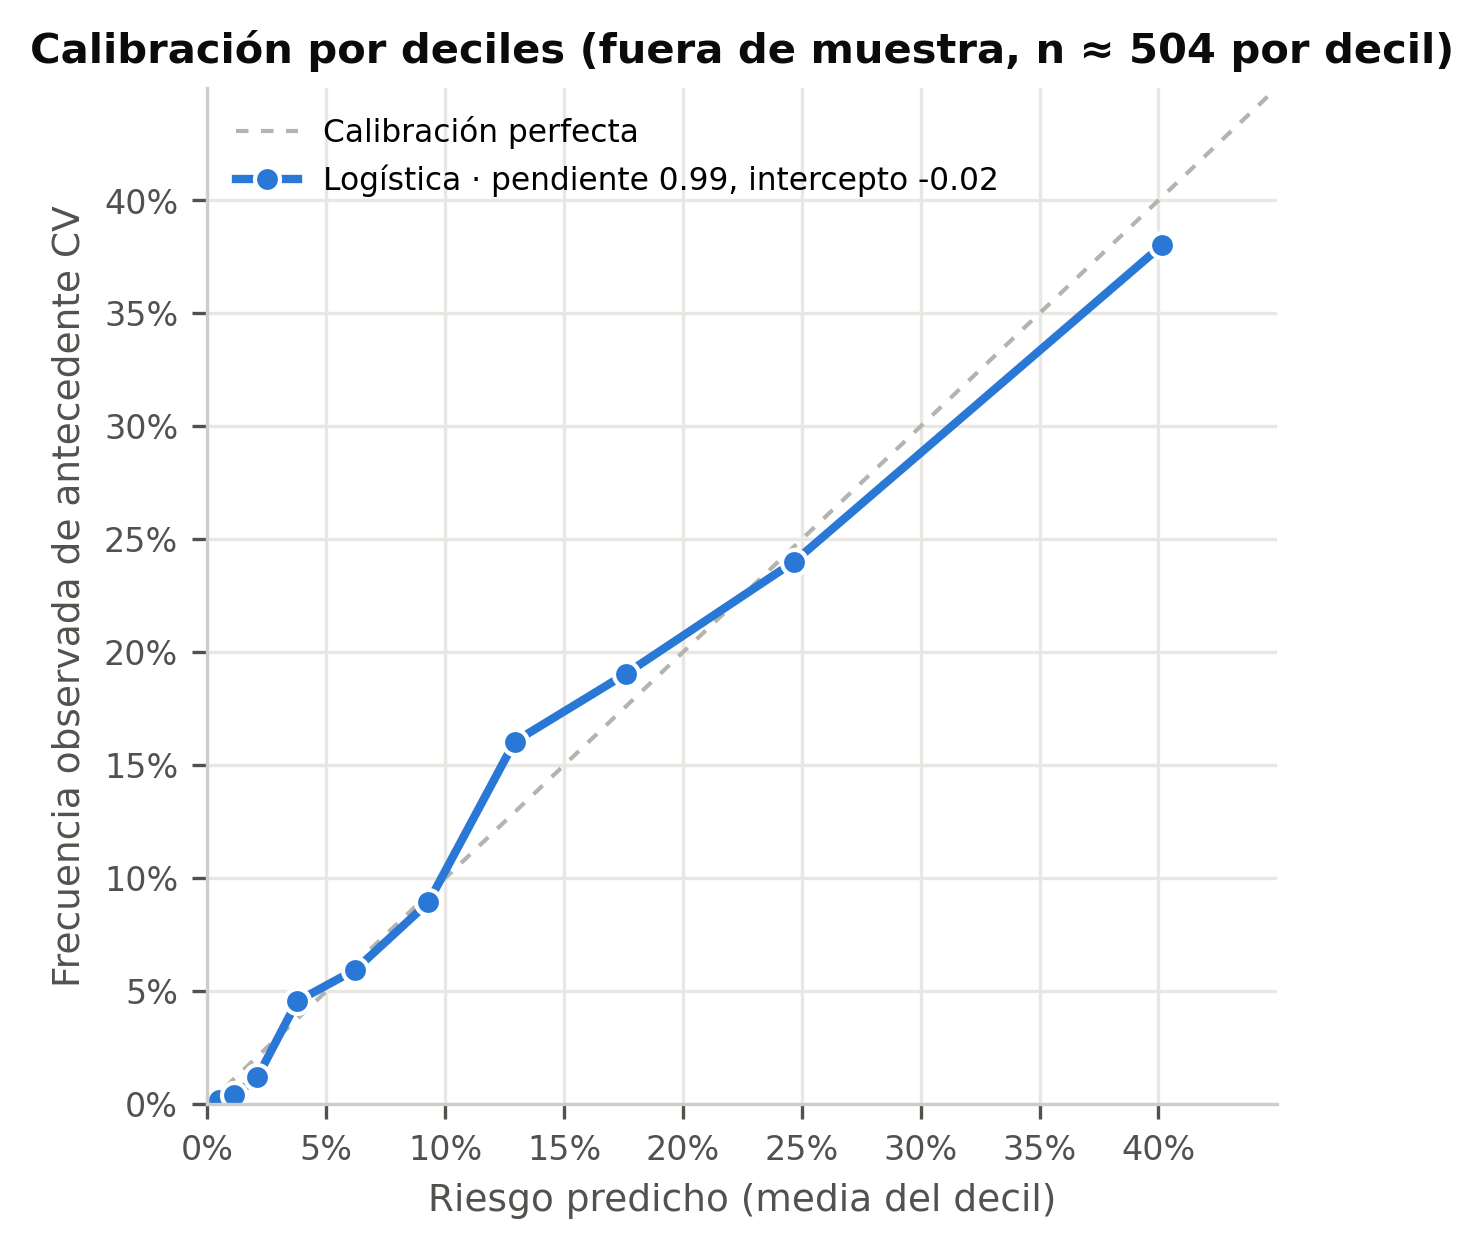
\includegraphics[width=\columnwidth]{../figuras/fig10-calibracion-nhanes.png}
\caption{Calibración por deciles de riesgo predicho de la regresión logística con estilo de vida, edad y sexo, resultado preliminar. Elaboración propia.}
\end{figure}
\begin{table*}[!t]
\centering
\caption{Odds ratio de la regresión logística seleccionada (resultado preliminar)}
\footnotesize
\renewcommand{\arraystretch}{1.15}
\begin{tabular}{>{\raggedright\arraybackslash}p{0.210\linewidth}>{\raggedright\arraybackslash}p{0.253\linewidth}>{\raggedright\arraybackslash}p{0.257\linewidth}>{\raggedright\arraybackslash}p{0.150\linewidth}}
\hline
\textbf{Variable} & \textbf{OR por 1 DE (IC 95 \%)} & \textbf{OR por unidad (IC 95 \%)} & \textbf{Unidad} \\ \hline
Edad & 4{,}06 (3{,}51–4{,}69) & 2{,}27 (2{,}09–2{,}47) & +10 años \\ \hline
Índice de masa corporal & 1{,}46 (1{,}33–1{,}60) & 1{,}30 (1{,}22–1{,}39) & +5 kg/m$^{2}$ \\ \hline
Sexo masculino & 1{,}41 (1{,}28–1{,}55) & 2{,}00 (1{,}65–2{,}41) & Hombre frente a mujer \\ \hline
PHQ-9 & 1{,}39 (1{,}27–1{,}52) & 1{,}43 (1{,}30–1{,}57) & +5 puntos \\ \hline
Fumador actual & 1{,}24 (1{,}14–1{,}35) & 1{,}85 (1{,}44–2{,}37) & Sí frente a no \\ \hline
Horas de sueño & 1{,}14 (1{,}04–1{,}24) & 1{,}09 (1{,}03–1{,}15) & +1 hora \\ \hline
Frecuencia cardíaca en reposo & 1{,}11 (1{,}01–1{,}21) & 1{,}08 (1{,}01–1{,}17) & +10 lpm \\ \hline
\end{tabular}
\par\smallskip\parbox{\linewidth}{\scriptsize\textit{Nota:} DE: desvío estándar. Todos los coeficientes tienen p < 0{,}05. El odds ratio del sueño es positivo porque el sueño largo también se asocia con mayor riesgo y, en un diseño transversal, está confundido por la edad y la morbilidad previa. Elaboración propia.}
\end{table*}
Esta tabla reemplaza la figura de importancia de variables: además de ordenar las variables, muestra la magnitud de cada asociación con su incertidumbre. Para un usuario concreto, la aplicación ordena sus variables según el valor SHAP exacto; por ejemplo, para una persona con índice de masa corporal alto y sin tabaquismo, indica que el índice de masa corporal es la variable modificable que más aumenta su riesgo frente al promedio y que no fumar lo reduce, lo que orienta directamente las recomendaciones de alimentación y ejercicio.

Del lado del desarrollo: el número de historias de usuario completadas frente a las planeadas, el resultado de las pruebas unitarias y de integración con su cobertura, y la evidencia de funcionamiento de cada módulo mediante capturas de pantalla del prototipo.

Toda métrica se reporta acompañada del tamaño del conjunto sobre el que se calculó. Un valor de exactitud sin el número de casos de prueba no constituye un resultado verificable.

\subsection{Resultados del tercer objetivo específico}
Se reportan los resultados de la validación en cuatro bloques. El primero corresponde a la usabilidad: puntaje promedio del cuestionario con su desviación estándar y el número de participantes, la distribución de puntajes individuales y el valor obtenido del coeficiente alfa de Cronbach. El segundo corresponde al desempeño en tarea: tasa de finalización, tiempo promedio y número de errores por cada tarea evaluada, presentados en tabla. El tercero corresponde a la auditoría técnica: puntajes obtenidos en rendimiento, accesibilidad y cumplimiento de criterios de aplicación web progresiva, y el resultado de la verificación de los controles de seguridad, indicando el nivel de cumplimiento por categoría. El cuarto corresponde a la revisión clínica: los hallazgos del profesional de salud, clasificados por severidad y acompañados del ajuste realizado en respuesta a cada uno.

Se reporta también el comportamiento del sistema sin conexión, indicando qué funcionalidades permanecieron disponibles, si la persistencia local operó correctamente y si la sincronización se completó al restablecer la red.

\begin{table*}[!t]
\centering
\caption{Criterios de aceptación de la aplicación}
\footnotesize
\renewcommand{\arraystretch}{1.15}
\begin{tabular}{>{\raggedright\arraybackslash}p{0.110\linewidth}>{\raggedright\arraybackslash}p{0.641\linewidth}>{\raggedright\arraybackslash}p{0.151\linewidth}}
\hline
\textbf{Aspecto} & \textbf{Criterio de aceptación} & \textbf{Instrumento} \\ \hline
Usabilidad percibida & Puntaje SUS medio $\geq$ 70, cercano a la media reportada en la literatura [27] & Escala SUS \\ \hline
Autonomía & Al menos el 80 \% de los participantes completa la primera evaluación sin asistencia & Registro de tareas \\ \hline
Operación sin conexión & La última evaluación con su explicación, el plan, las rutinas y el histórico se consultan en modo avión en todos los dispositivos de prueba & Lista de verificación técnica \\ \hline
Rendimiento & Primera carga útil en menos de 3 s con 3G simulada y resultado del riesgo en menos de 2 s con conexión & Lighthouse y registro del servidor \\ \hline
Pertinencia clínica & Sin observaciones críticas del profesional sobre categorías de riesgo y mensajes de derivación & Entrevista semiestructurada \\ \hline
\end{tabular}
\par\smallskip\parbox{\linewidth}{\scriptsize\textit{Nota:} elaboración propia.}
\end{table*}
\subsection{Formato de presentación}
Las tablas y figuras se numeran de forma consecutiva y llevan un rótulo que describe su contenido. Cada una se referencia en el texto antes de aparecer. Los resultados negativos o inferiores a lo esperado se reportan con el mismo detalle que los favorables, dado que un instrumento que arroja un valor bajo de confiabilidad o un modelo que no alcanza la sensibilidad requerida constituyen hallazgos válidos y su omisión comprometería la integridad del trabajo.

\section{Conclusiones}
El análisis desarrollado permite concluir que el problema de las enfermedades cardiovasculares en Colombia no se explica por un déficit de conocimiento clínico, sino por una falla en el momento de la detección. El tamizaje disponible depende de que la persona asista a consulta, de modo que quien no consulta permanece sin evaluar hasta que ocurre un evento agudo. Esta condición, combinada con la desigualdad territorial en el acceso a servicios preventivos y a conectividad estable, define una brecha que admite intervención desde la ingeniería de sistemas.

La revisión de antecedentes muestra que los componentes técnicos necesarios existen y están validados de forma aislada: modelos de aprendizaje automático que igualan o superan a las escalas de riesgo tradicionales, nutrición personalizada con evidencia clínica medible, sistemas de recomendación de actividad física con mayor adherencia que las prescripciones genéricas y arquitecturas de aplicación web progresiva probadas en contextos de salud pública. El vacío no está en los componentes sino en su articulación, y ese es el aporte que propone Pulso.

La elección de una arquitectura de Aplicación Web Progresiva responde de manera directa a las restricciones del contexto colombiano. La consulta sin conexión mediante Service Workers, el almacenamiento local con IndexedDB y la instalación sin dependencia de tiendas de aplicaciones no son decisiones estéticas, sino la respuesta técnica a la conectividad intermitente y a los dispositivos de gama baja que predominan en la población con mayor barrera de acceso.

La definición del modelo resulta igualmente determinante. La comparación sobre NHANES 2021-2023 muestra que una regresión logística con las variables de estilo de vida, la edad y el sexo alcanza un área bajo la curva ROC de 0{,}805, bien calibrada, y que gradient boosting y k vecinos más cercanos no la superan. Al ser lineal, el modelo permite calcular de forma exacta el valor SHAP de cada variable en el mismo instante de la predicción; la explicación se guarda con la evaluación y queda disponible sin conexión, lo que resuelve la tensión entre explicabilidad y operación sin red. Dado que la literatura señala la escasa validación externa y el carácter de caja negra de los modelos como obstáculos principales para su adopción [4], un resultado auditable por el usuario y por el profesional de salud constituye una condición de confianza y no un añadido opcional.

Finalmente, el proyecto reconoce de forma explícita los límites de su alcance. El conjunto de entrenamiento proviene de población estadounidense y no colombiana, su diseño transversal no permite estimar incidencia futura, las recomendaciones tienen carácter orientativo y no sustituyen el criterio médico profesional, una evaluación nueva requiere conexión y el sistema opera por evaluación periódica y no por monitoreo continuo. La validación con datos poblacionales colombianos y la revisión clínica del prototipo quedan planteadas como condición para cualquier uso más allá del ámbito académico, y como línea natural de trabajo posterior.


\begin{thebibliography}{99}
\bibitem{r1} Ministerio de Salud y Protección Social de Colombia, "Análisis de Situación de Salud (ASIS) Colombia," Bogotá, Colombia, 2022. [En línea]. Disponible en: \url{https://www.minsalud.gov.co}
\bibitem{r2} Organización Mundial de la Salud, "Enfermedades cardiovasculares," Nota descriptiva, 2025. [En línea]. Disponible en: \url{https://www.who.int/es/news-room/fact-sheets/detail/cardiovascular-diseases-(cvds)}
\bibitem{r3} World Heart Federation, "World Heart Report 2023: Confronting the world's number one killer," Ginebra, Suiza, 2023. [En línea]. Disponible en: \url{https://world-heart-federation.org/wp-content/uploads/World-Heart-Report-2023.pdf}
\bibitem{r4} C. Krittanawong et al., "Machine learning prediction in cardiovascular diseases: A meta-analysis," Sci. Rep., vol. 10, no. 1, Art. no. 16057, 2020, doi: 10.1038/s41598-020-72685-1.
\bibitem{r5} S. F. Weng, J. Reps, J. Kai, J. M. Garibaldi y N. Qureshi, "Can machine-learning improve cardiovascular risk prediction using routine clinical data?," PLoS ONE, vol. 12, no. 4, Art. no. e0174944, 2017, doi: 10.1371/journal.pone.0174944.
\bibitem{r6} SCORE2 working group and ESC Cardiovascular risk collaboration, "SCORE2 risk prediction algorithms: New models to estimate 10-year risk of cardiovascular disease in Europe," Eur. Heart J., vol. 42, no. 25, pp. 2439–2454, 2021, doi: 10.1093/eurheartj/ehab309.
\bibitem{r7} D. Zeevi et al., "Personalized nutrition by prediction of glycemic responses," Cell, vol. 163, no. 5, pp. 1079–1094, 2015, doi: 10.1016/j.cell.2015.11.001.
\bibitem{r8} P. Liao, K. Greenewald, P. Klasnja y S. Murphy, "Personalized HeartSteps: A reinforcement learning algorithm for optimizing physical activity," Proc. ACM Interact. Mob. Wearable Ubiquitous Technol., vol. 4, no. 1, 2020, doi: 10.1145/3381007.
\bibitem{r9} D. Biduski, E. A. Bellei, J. P. M. Rodriguez, L. A. M. Zaina y A. C. B. De Marchi, "Assessing long-term user experience on a mobile health application through an in-app embedded conversation-based questionnaire," Comput. Hum. Behav., vol. 104, Art. no. 106169, 2020, doi: 10.1016/j.chb.2019.106169.
\bibitem{r10} Centers for Disease Control and Prevention, National Center for Health Statistics, "National Health and Nutrition Examination Survey: August 2021 – August 2023 data files," U.S. Department of Health and Human Services, Hyattsville, MD, EE. UU., 2024. [En línea]. Disponible en: \url{https://wwwn.cdc.gov/nchs/nhanes/continuousnhanes/default.aspx?Cycle=2021-2023}
\bibitem{r11} A. Janosi, W. Steinbrunn, M. Pfisterer y R. Detrano, "Heart Disease," UCI Machine Learning Repository, 1988, doi: 10.24432/C52P4X.
\bibitem{r12} R. B. D'Agostino et al., "General cardiovascular risk profile for use in primary care: The Framingham Heart Study," Circulation, vol. 117, no. 6, pp. 743–753, 2008, doi: 10.1161/CIRCULATIONAHA.107.699579.
\bibitem{r13} K. Kroenke, R. L. Spitzer y J. B. W. Williams, "The PHQ-9: Validity of a brief depression severity measure," J. Gen. Intern. Med., vol. 16, no. 9, pp. 606–613, 2001, doi: 10.1046/j.1525-1497.2001.016009606.x.
\bibitem{r14} S. M. Lundberg y S.-I. Lee, "A unified approach to interpreting model predictions," en Advances in Neural Information Processing Systems 30, 2017, pp. 4765–4774.
\bibitem{r15} J. Brooke, "SUS: A 'quick and dirty' usability scale," en Usability Evaluation in Industry, P. W. Jordan, B. Thomas, B. A. Weerdmeester e I. L. McClelland, Eds. Londres, Reino Unido: Taylor \& Francis, 1996, pp. 189–194.
\bibitem{r16} R. Detrano et al., "International application of a new probability algorithm for the diagnosis of coronary artery disease," Amer. J. Cardiol., vol. 64, no. 5, pp. 304–310, 1989, doi: 10.1016/0002-9149(89)90524-9.
\bibitem{r17} B. Van Calster, D. J. McLernon, M. van Smeden, L. Wynants y E. W. Steyerberg, "Calibration: The Achilles heel of predictive analytics," BMC Med., vol. 17, Art. no. 230, 2019, doi: 10.1186/s12916-019-1466-7.
\bibitem{r18} T. Hastie, R. Tibshirani y J. Friedman, The Elements of Statistical Learning: Data Mining, Inference, and Prediction, 2.ª ed. Nueva York, NY, EE. UU.: Springer, 2009, doi: 10.1007/978-0-387-84858-7.
\bibitem{r19} S. le Cessie y J. C. van Houwelingen, "Ridge estimators in logistic regression," J. Roy. Statist. Soc. Ser. C (Appl. Statist.), vol. 41, no. 1, pp. 191–201, 1992, doi: 10.2307/2347628.
\bibitem{r20} J. H. Friedman, "Greedy function approximation: A gradient boosting machine," Ann. Statist., vol. 29, no. 5, pp. 1189–1232, 2001, doi: 10.1214/aos/1013203451.
\bibitem{r21} T. Cover y P. Hart, "Nearest neighbor pattern classification," IEEE Trans. Inf. Theory, vol. 13, no. 1, pp. 21–27, 1967, doi: 10.1109/TIT.1967.1053964.
\bibitem{r22} L. Breiman, "Random forests," Mach. Learn., vol. 45, no. 1, pp. 5–32, 2001, doi: 10.1023/A:1010933404324.
\bibitem{r23} T. Chen y C. Guestrin, "XGBoost: A scalable tree boosting system," en Proc. 22nd ACM SIGKDD Int. Conf. Knowledge Discovery and Data Mining, 2016, pp. 785–794, doi: 10.1145/2939672.2939785.
\bibitem{r24} J. A. Hanley y B. J. McNeil, "The meaning and use of the area under a receiver operating characteristic (ROC) curve," Radiology, vol. 143, no. 1, pp. 29–36, 1982, doi: 10.1148/radiology.143.1.7063747.
\bibitem{r25} W. J. Youden, "Index for rating diagnostic tests," Cancer, vol. 3, no. 1, pp. 32–35, 1950.
\bibitem{r26} B. Efron y R. J. Tibshirani, An Introduction to the Bootstrap. Nueva York, NY, EE. UU.: Chapman \& Hall, 1993.
\bibitem{r27} A. Bangor, P. T. Kortum y J. T. Miller, "An empirical evaluation of the System Usability Scale," Int. J. Hum.-Comput. Interact., vol. 24, no. 6, pp. 574–594, 2008, doi: 10.1080/10447310802205776.
\end{thebibliography}
\end{document}
